
\newpage
\begin{tikzpicture}[remember picture, overlay]
	\node [inner sep=0pt, minimum width=\paperwidth, minimum height=\paperheight,opacity=1,color=Apricot] at (current page.center) {
\includegraphics[width=\paperwidth,height=\paperheight,angle=0]{paper18}};
	\node [xscale=1,inner sep=0pt,xshift=-.32\paperwidth,yshift=-.28\paperheight] at (current page.center) {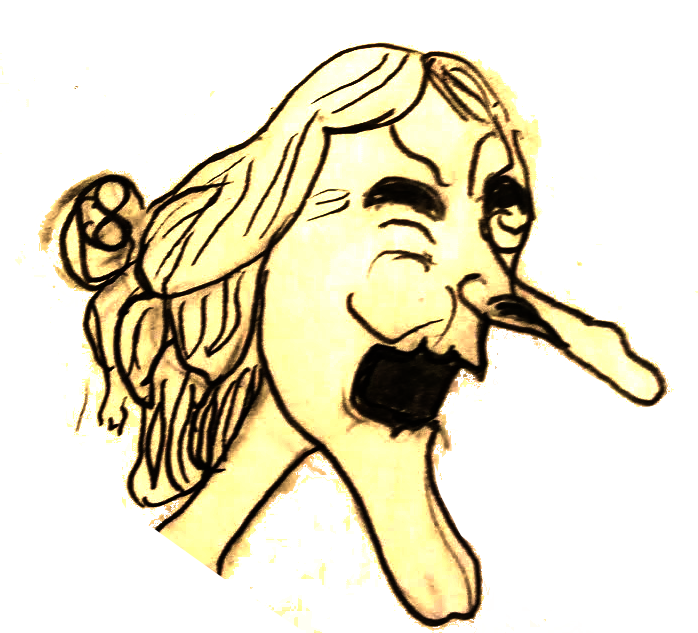
\includegraphics[width=.3\paperwidth,angle=0]{biglia1.png}};
\end{tikzpicture}
COMENZÓ A SUBIR UNA AMPLIA ESCALERA DE MÁRMOL MUY SUAVE, DE PELDAÑOS DE PLACAS REDONDEADAS.  LE LLAMAN TAMBIÉN ESCALERA CARACOL POR LA FORMA ESPIRALADA QUE TIENEN ESAS BABOSAS EN SUS CAPARAZONES. EL MÁRMOL ERA VISIBLE POR SU BLANCURA, CUALQUIER TENUE RAYO DE LUZ SERVÍA PARA ILUMINARLO. SIENDO TAN CLARO, BORIS SUBIÓ CÓMODO, CONFIADO EN CONFUNDIR SU CORTO PELAJE CON LOS ESCALONES.
UNA TENUE LUZ TEMBLOROSA, COMO LAS QUE VIENEN DE LAS VELAS, SE PERCIBÍA EN EL NIVEL SUPERIOR.

CUANDO BORIS LLEGÓ TRANQUILO, VICTORIOSO DONDE QUERÍA,

\begin{flushright}
	UNA INESPERADA PRESENCIA  LO SORPRENDIÓ  DESDE 
	
	ATRÁS. 
	SE TRATABA DE UNA ANCIANA SEÑORA,  
	VESTIDA 
	
	DE 
	BLANCO,    LO TOMÓ POR 
	EL  
	CUELLO Y EXCLAMÓ:
	
	- ¿ Y ADONDE CREÉS QUE VAS, PEQUEÑÍN? 	
\end{flushright}
\newpage
\begin{tikzpicture}[remember picture, overlay]
	\node [inner sep=0pt, minimum width=\paperwidth, minimum height=\paperheight,opacity=.2,color=Red,fill=Green0] at (current page.center){};
	\node [inner sep=0pt, minimum width=\paperwidth, minimum height=\paperheight,opacity=.5] at (current page.center) {
\includegraphics[width=\paperwidth,height=\paperheight,angle=180]{paper18}};
	\node [xscale=1,inner sep=0pt,xshift=-.1\paperwidth,yshift=-.28\paperheight] at (current page.center) {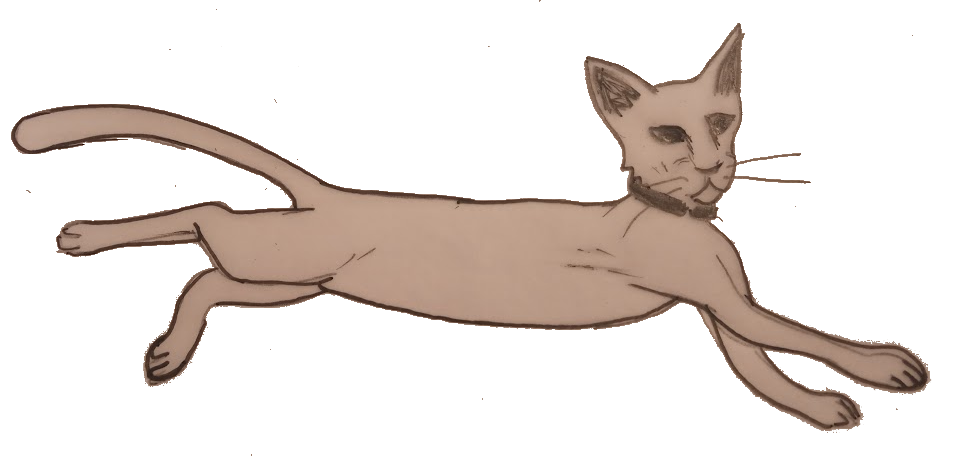
\includegraphics[width=.6\paperwidth,angle=0]{boris2.png}};
\end{tikzpicture}
SINTIÓ EL AGARRE FRÍO Y FANTASMAL DE LA SEÑORA Y PEGÓ UN SALTO QUE LO PUSO A SALVO. CUALQUIER OTRO HUBIESE COMENZADO UNA CARRERA FRENÉTICA POR EL VESTÍBULO DEL SEGUNDO PISO DEL CASTILLO PERO ÉL PREFIRIÓ OBSERVAR A LA ANCIANA DESDE UNA DISTANCIA PRUDENTE.

PARECÍA ELLA DE UNA EDAD MUY AVANZADA, TENÍA EL PELO REVUELTO Y ESTABA VESTIDA TODA DE BLANCO. ERA MUY PÁLIDA, Y SI BIEN AL PRINCIPIO BORIS HABÍA SENTIDO MIEDO, PUDO OBSERVAR QUE SU ROSTRO ERA MÁS BIEN TRISTE QUE ENOJADO.

\newpage
\begin{tikzpicture}[remember picture, overlay]
	\node [inner sep=0pt, minimum width=\paperwidth, minimum height=\paperheight,opacity=.3,color=Red,fill=Red1] at (current page.center){};
	\node [inner sep=0pt, minimum width=\paperwidth, minimum height=\paperheight,opacity=.15] at (current page.center) {
\includegraphics[width=\paperwidth,height=\paperheight,angle=180]{paper18}};
\end{tikzpicture}

LA SEÑORA BIGLIA LE HABLÓ AL GATO COMO SI SE TRATARA DE UNA PERSONA.

- QUERIDO, PUEDO ESCUCHAR TUS PENSAMIENTOS, SÉ POR QUÉ HAS VENIDO.

CARAMBA!, PENSÓ BORIS.

- AHÍ POR TU CABEZA, PASÓ LA EXPRESIÓN ´´CARAMBA´´

- ES USTED EXTRAORDINARIA, LE DIJO FINALMENTE BORIS, ¿CÓMO LO HACE?

- SOY COMO UN FANTASMA, Y LOS GATOS ME OYEN Y PUEDEN COMUNICAR CONMIGO. 

- ¿ES CIERTO ENTONCES QUE EXISTE UNA MALDICIÓN SOBRE ESTA CASA DE PIEDRA?
\newpage
\begin{tikzpicture}[remember picture, overlay]
	\node [inner sep=0pt, minimum width=\paperwidth, minimum height=\paperheight,opacity=.3,color=Red,fill=Red1] at (current page.center){};
	\node [inner sep=0pt, minimum width=\paperwidth, minimum height=\paperheight,opacity=.15] at (current page.center) {
\includegraphics[width=\paperwidth,height=\paperheight,angle=180]{paper18}};
\end{tikzpicture}
- LA VERDAD ES QUE NO ME ACUERDO, DESPERTÉ UN DÍA EN MI HABITACIÓN Y NO PUEDO SALIR DEL CASTILLO, CADA VEZ QUE LO HAGO, VUELVO A DESPERTAR EN EL MISMO LUGAR.

BORIS SE HIZO PRONTO AMIGO DE LA SEÑORA Y FUE LA ÚLTIMA VEZ QUE SE LE VIÓ FUERA DEL PALACIO DE LOS BICHOS. Y ASÍ TERMINA LA HISTORIA, OTTOKO.

- PERO, ¡CÓMO ES POSIBLE! ¡QUEDAN MUCHAS PREGUNTAS POR CONTESTAR!, PROTESTÉ. -POR EMPEZAR, ¿CÓMO ES QUE USTEDES DOS CONOCEN LA HISTORIA?

- PORQUE SI BIEN TE DIJE QUE BORIS NUNCA SALIÓ DE ALLÍ, SI LO HICIERON LOS HIJOS DE BORIS Y MELISSA. Y DE TALES GATOS NEGROS Y BLANCOS SALIERON HERMOSOS GATOS GRISES, JIJIJI.

- ENTONCES, ¿USTEDES?

MIRÉ A DORA Y A MORA COMPLETAMENTE ASOMBRADO.

\newpage
\begin{tikzpicture}[remember picture, overlay]
	\node [inner sep=0pt, minimum width=\paperwidth, minimum height=\paperheight,opacity=.8,color=Apricot] at (current page.center) {
\includegraphics[width=\paperwidth,height=\paperheight,angle=0]{paper26}};
	\node [xscale=1,inner sep=0pt,xshift=.4\paperwidth,yshift=.4\paperheight] at (current page.center) {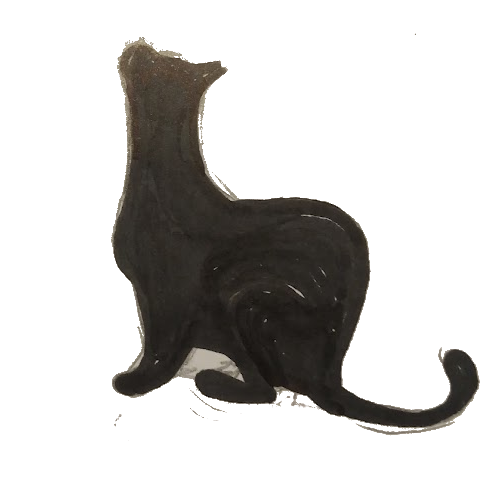
\includegraphics[width=.15\paperwidth,angle=0]{ottoko_atento.png}};	
\end{tikzpicture}
ASÍ SUPE QUE MIS DOS AMIGAS ERAN DESCENDIENTES DE 

MELISSA Y BORIS, GRAN ALCURNIA FELINA DE VILLA DEL

 PARQUE. Y MELISSA HABÍA SIDO LA GATA DE AMELIA, AUNQUE QUEDABAN MUCHAS COSAS MISTERIOSAS POR DEVELAR.
 
 NO PUDE DEJAR DE SOÑAR CON LAS ESCALERAS Y LOS COQUETOS PISOS DEL CASTILLO. HOY DÍA ESTABA TODO RESTAURADO, CON ALGUNOS AGREGADOS Y CIERTAS AUSENCIAS. DESDE EL EXTERIOR, YA NO SE VEN GÁRGOLAS SOBRE LAS PAREDES. Y VARIAS PERSONAS REALES Y NINGÚN FANTASMA HABITAN LOS DISTINTOS NIVELES DEL EDIFICIO.
 
 ¿QUEDARÍA ALGO DE LA MAGIA DE ANTAÑO? ¿O EN NUESTROS TIEMPOS TODOS LOS SECRETOS HAN DESAPARECIDO?
 
 ¿HA PERDIDO SU ALMA EN SU MODERNA RENOVACIÓN EL CASTILLO?
 
 MORA ME RECORDÓ QUE HABÍA ALGO DENTRO DEL EDIFICIO QUE PROBABA SU HISTORIA, EL COLLAR DE BORIS. ALGUIEN PODRÍA RECUPERARLO.
%, LOS OJOS ABIERTOS GRANDES Y LA PUPILA ALGO DILATADA.
%  